% 3.1.PrepareApplication.tex
%	Last update: 2019/10/03 F.Kanehori
%\newpage
\subsection{準備}
\label{subsec:PrepareApplication}

\noindent
アプリケーションと並行してSpringheadライブラリを開発する場合には、
\KQuoteS\ref{subsec:Problems} CMakeを使用した場合の問題点\KQuoteE
で示した問題に対処する必要があるため、
ここで述べる方法に従って作業を進めてください
(\KQuote{\ref{subsec:Solution} 対処法}で示した方策が組み込まれます)。

\medskip
以下、Springheadライブラリをダウンロードしたディレクトリを\SprTop{} 、
アプリケーションプログラムを作成するディレクトリを\AppTop{}として説明を進めます。

\bigskip
\noindent
\AppTop{}に移動してください。

\bigskip
\noindent
配布されたファイル\CMakeTopdir{.dist}を\CMakeTopdir{}という名前で、
\CMakeLists{.Dev.dist}を\CMakeLists{}という名前でコピーします
(誤コミットを防止するためにもリネームではなくコピーしてください)。

\medskip
\ifLwarp
	\begin{figure}[h]
	    \begin{center}
	    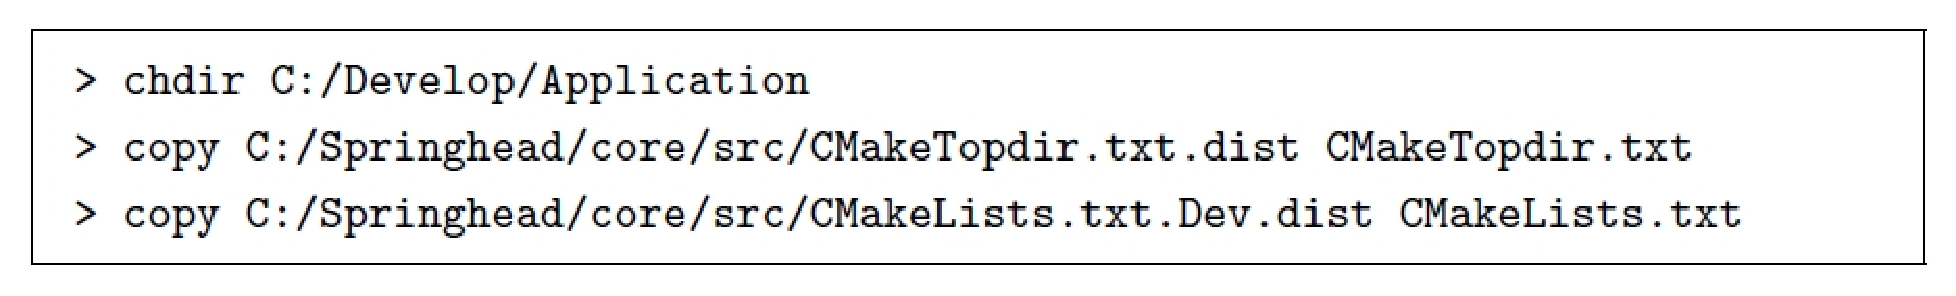
\includegraphics[width=\textwidth]{fig/command-3-1-a.eps}
	    \end{center}
	    \label{fig:DownloadTree}
	\end{figure}
\else
\begin{narrow}[15pt]
	\CmndBox{%
	{\small{> chdir C:/Develop/Application}}\\
	{\small{> copy C:/Springhead/core/src/CMakeTopdir.txt.dist CMakeTopdir.txt}}\\
	{\small{> copy C:/Springhead/core/src/CMakeLists.txt.Dev.dist CMakeLists.txt}}
	}
\end{narrow}
\fi

\bigskip
\noindent
\bf{\CMakeTopdir{}}の編集
\begin{narrow}[20pt]
	\CMakeTopdir{}には\SprLib をダウンロードしたディレクトリを設定します。
	これは、CMakeにSpringheadのソースツリーの場所を教えるために必要な設定です。

\ifLwarp
	\begin{figure}[h]
	    \begin{center}
	    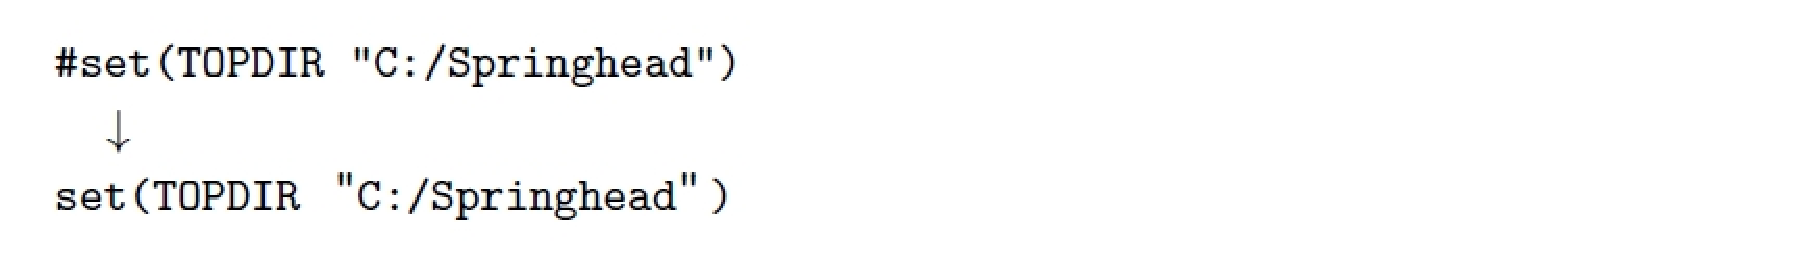
\includegraphics[width=\textwidth]{fig/command-3-1-b.eps}
	    \end{center}
	    \label{fig:DownloadTree}
	\end{figure}
\else
	\begin{narrow}[15pt]
		\CmndBox{%
			{\small{\#set(TOPDIR "C:/Springhead")}}\\
			\hspace{10pt}{\small{$\downarrow$}}\\
			{\small{set(TOPDIR \SprTop{})}}
		}
	\end{narrow}
\fi
\end{narrow}
\medskip
\noindent
\bf{\CMakeLists{}}の編集
\begin{narrow}[20pt]
	\begin{enumerate}
	    \item
		プロジェクト名を設定します(11行目)。

\ifLwarp
		\begin{figure}[h]
			\begin{center}
			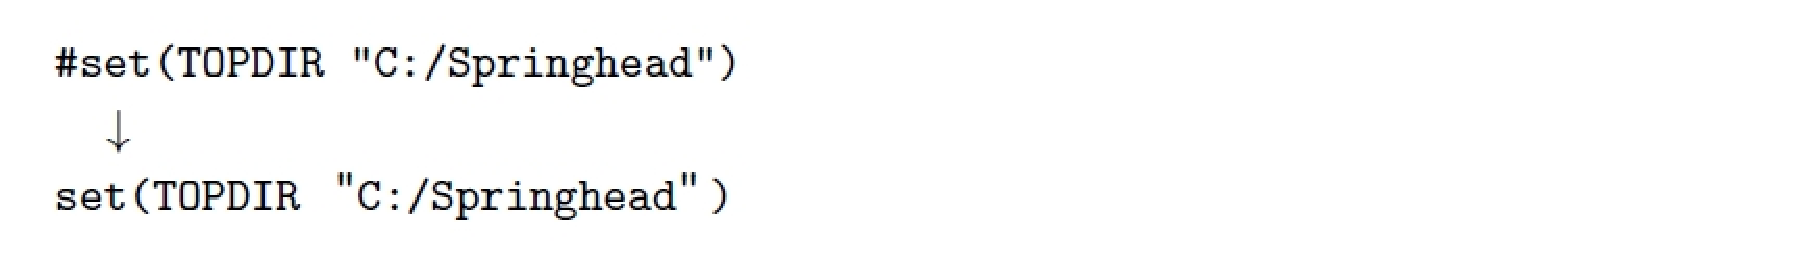
\includegraphics[width=\textwidth]{fig/command-3-1-b.eps}
				\end{center}
			\label{fig:DownloadTree}
		\end{figure}
\else
		\begin{narrow}[s][5pt]
			\CmndBox{%
				{\small{set(ProjectName "Project")}}\\
				\hspace{10pt}{\small{$\downarrow$}}\\
				{\small{set(ProjectName "<\it{MyApplication}>")}}
			}
		\end{narrow}
		\Vskip{.5\baselineskip}
\fi

	    \item
		Customization section (19行目以降)を必要に応じて変更します。\\
		各変数の意味は次のとおりです。

		\medskip
		\def\SetRelPath{\tt{RELATIVE \$\{CMAKE\_SOURCE\_DIR\}}}
		\def\CMakeSrcDir{\tt{\$\{CMAKE\_SOURCE\_DIR\}}}
		\begin{narrow}[4pt]
		\begin{tabular}{|l|l|}\hline
		    \tt{OOS\_BLD\_DIR} &
			CMakeの作業領域(ディレクトリ)の名前(本ドキュ\\
			& メントで\build としているもの)。\\\hline
		    \multicolumn{2}{|l|}{%
			\tt{CMAKE\_CONFIGURATION\_TYPES}} \\
			& ビルド構成。\\\hline
		    \tt{SRCS} &
			ビルドの対象とするファイル。
			設定は\tt{set(SRCS …)} \\
			& または\tt{file(GLOB SRCS …)}とします。\\
			& 後者ではワイルドカードが使えます。\\
			& \tt{SRCS}の直後に``\tt{RELATIVE <\it{base-dir}>}''を付加すると \\
			& 相対パス指定となります。デフォルトは \\
			& \ \ {\footnotesize{\tt{file(GLOB \SetRelPath\ *.cpp *.h)}}} \\
			& です。\\\hline
		    \tt{EXCLUDE\_SRCS} &
			ビルドの対象から外すファイル。\\
			& 上の\tt{SRCS}で\tt{RELATIVE}としていないときは絶対パス \\
			& で指定します。\\
			& \tt{SRCS}でワイルドカードを使用した場合に有用です。\\\hline
		    \tt{SPR\_PROJS} &
			アプリケーションに組み込むSpringheadライブラリ\\
			& のプロジェクト名。\\
			& 不要なプロジェクト名を削除します。
			この中にRun-\\
			& Swigを含めてはいけません。\\\hline
		    \tt{ADDITIONAL\_INCDIR} &
			追加のインクルードパス指定。\\
			& 現在のディレクトリは \CMakeSrcDir で参照 \\
			& できます。\\\hline
		    \tt{ADDITIONAL\_LIBDIR} &
			追加のライブラリパス指定。\\\hline
		    \tt{ADDITIONAL\_LIBS} &
			追加のライブラリファイル名。\\\hline
		    \tt{EXCLUDE\_LIBS} &
			linkの対象から外すライブラリファイル名。\\
			& デフォルトで組み込まれてしまうライブラリファイル\\
			& を排除するために指定します。\\\hline
\ifLwarp\else
		\end{tabular}
		\begin{tabular}{|l|l|}\hline
\fi
		    \multicolumn{2}{|l|}{%
			\tt{DEBUGGER\_WORKING\_DIRECTORY}} \\
			\phantom{\tt{ADDITIONAL\_LIBDIR}}
			& Visual Studio Debuggerの作業ディレクトリ名。\\
			& デバッガはこのディレクトリで起動されたように振る \\
			& 舞います。\\\hline
		    \multicolumn{2}{|l|}{%
			\tt{DEBUGGER\_COMMAND\_ARGUMENTS}} \\
			& Visual Studio Debuggerに渡すコマンド引数 \\\hline
		\end{tabular}
		\end{narrow}
	\end{enumerate}
\end{narrow}

\bigskip
\noindent
自前でインストールしているパッケージ
(\tt{boost}, \tt{glew}, \tt{freeglut}, \tt{glui})を使用する場合には、
さらに、
配布されたファイル\CMakeConf{.dist}を\CMakeConf{}という名前でコピーして
必要な編集をします。
\KQuote{\ref{subsec:PrepareLibrary} 準備}を参照してください。

\medskip
\noindent
ビルドの条件(compile/linkのパラメータ)を変更したいときは、
配布されたファイル\CMakeOpts{.dist}を\CMakeOpts{}という名前でコピーして
適宜変更してください。

\medskip
\noindent
以上で準備作業は終了です。

% end: 3.1.PrepareApplication.tex
